
\documentclass{beamer}


\mode<presentation>{
  % \useinnertheme{rectangles}
  \useoutertheme{infolines}
  % \usecolortheme{crane}
  % \usecolortheme{rose}
}
%% Pre-amble - commonly defined macros.

%% Packages
\usepackage{fixltx2e}
\usepackage{amsmath}
\usepackage{amsfonts}
\usepackage{amssymb}
\usepackage{amsbsy}
\usepackage{isomath}
\usepackage{amsthm}
\usepackage{dsfont}
%%\usepackage{theorem}
\usepackage{algorithm}
\usepackage{algorithmicx}
\usepackage{algpseudocode}
\usepackage{mathrsfs}
\usepackage{epsfig}
\usepackage{subcaption}
\usepackage{makeidx} 
\usepackage{colortbl}
\usepackage{enumerate}
\usepackage{multirow}
\usepackage{listings}
\usepackage{pgfplots}
\usepackage{fontawesome}
\newlength\fheight
\newlength\fwidth
\only<presentation>{
\setlength\fheight{\textheight}
\setlength\fwidth{0.45\columnwidth}
}
\only<article>{
\setlength\fheight{0.25\textheight}
\setlength\fwidth{0.45\textwidth}
}
\usepackage[sort&compress,comma,super]{natbib}
\def\newblock{} % To avoid a compilation error about a function \newblock undefined
\usepackage{hyperref}

\newcommand \cdcomment[1] {\texttt{\color{red}[CD: #1]}}
  
\setbeamertemplate{theorems}[numbered] 
\mode<presentation>{
\theoremstyle{plain}
\newtheorem{assumption}{Assumption}
\theoremstyle{definition}
\newtheorem{exercise}{Exercise}
\theoremstyle{remark}
\newtheorem{remark}{Remark}
}

\numberwithin{equation}{section} 
\mode<article>{
  \theoremstyle{plain}
  % \newtheorem{assumption}{Assumption}[section]
  \newtheorem{lemma}{Lemma}[section]
  \newtheorem{theorem}{Theorem}[section]
  \newtheorem{corollary}{Corollary}[section]
  \theoremstyle{definition}
  \newtheorem{definition}{Definition}[section]
  \theoremstyle{remark}
  \newtheorem{remark}{Remark}[section]

  % \theoremstyle{plain} \newtheorem{remark}{Remark}[section]
  % \theoremstyle{plain} \newtheorem{definition}{Definition}[section]
  \theoremstyle{plain} \newtheorem{assumption}{Assumption}[section]
  
  %%% Examples %%%%
  \newtheoremstyle{example}  % Name
  {1em}       % Space above 
  {1em}       % Space below
  {\small}      % Body font
  {}          % Indent amount 
  {\scshape}  % Theorem head font
  {.}         % Punctuation after theorem head
  {.5em}      % Space after theorem head
  {}          % Theorem head spec
  \theoremstyle{example}
  \newtheorem{example}{Example}
  \newtheorem{exercise}{Exercise}

  \usepackage{framed}
  \usepackage[framemethod=tikz]{mdframed}
  \mdfsetup{%
    roundcorner=10pt}
  \renewenvironment{block}[1]
  {\begin{mdframed}[frametitle={#1}]}
    {\end{mdframed}}

  \renewenvironment{exampleblock}[1]
  {\begin{mdframed}[frametitle={\faGears{} #1}]}
    {\end{mdframed}}


  \renewenvironment{alertblock}[1]
  {\begin{mdframed}[backgroundcolor=red!20,frametitle={{\fontencoding{U}\fontfamily{futs}\selectfont\char 66\relax} #1}]}
    {\end{mdframed}}


  \newenvironment{theoryblock}[1]
  {\begin{mdframed}[backgroundcolor=yellow!20,frametitle={\Coffeecup #1}]}
    {\end{mdframed}}

  \newenvironment{exerciseblock}[1]
  {\begin{mdframed}[backgroundcolor=blue!10,frametitle={\faPencilSquareO{} #1}]}
    {\end{mdframed}}

  \newenvironment{groupactivity}[1]
  {\begin{mdframed}[backgroundcolor=cyan!20,frametitle={\faGroup{} #1}]}
    {\end{mdframed}}

  
}
%\theoremstyle{plain} \newtheorem{conjecture}{Conjecture}[section]
%\theoremstyle{plain} \newtheorem{theorem}{Theorem}[section]
%\theoremstyle{plain} \newtheorem{proposition}{Proposition}[section]
%\theoremstyle{plain} \newtheorem{lemma}{Lemma}[section]
%\theoremstyle{plain} \newtheorem{corollary}{Corollary}[section]


%\newenvironment{proof}[1][Proof]{\begin{trivlist}
%\item[\hskip \labelsep {\bfseries #1}]}{\end{trivlist}}
%\newcommand{\qed}{\nobreak \ifvmode \relax \else
%      \ifdim\lastskip<1.5em \hskip-\lastskip
%      \hskip1.5em plus0em minus0.5em \fi \nobreak
%      \vrule height0.5em width0.5em depth0.25em\fi}

\newcommand \indexmargin[1] {\marginpar{\emph{#1}}\index{#1}}
\newcommand \marginref[2] {\marginpar{\emph{#1}}\emph{#1}\index{#2}}
\newcommand \emindex[1] {\emph{#1}\marginpar{\emph{#1}}\index{#1}}


\newcommand \E {\mathop{\mbox{\ensuremath{\mathbb{E}}}}\nolimits}
\newcommand \hE {\hat{\mathop{\mbox{\ensuremath{\mathbb{E}}}}\nolimits}}
\renewcommand \Pr {\mathop{\mbox{\ensuremath{\mathbb{P}}}}\nolimits}
\newcommand \given {\mathrel{|}}
\newcommand \gvn {|}
\newcommand \eq {{=}}


%% Special characters
\newcommand\Reals {{\mathbb{R}}}
\newcommand\Naturals {{\mathbb{N}}} 
\newcommand\Simplex {\mathbold{\Delta}}

\newcommand \FB {{\mathfrak{B}}}
\newcommand \FD {{\mathfrak{D}}}
\newcommand \FF {{\mathfrak{F}}}
\newcommand \FM {{\mathfrak{M}}}
\newcommand \FK {{\mathfrak{K}}}
\newcommand \FJ {{\mathfrak{J}}}
\newcommand \FL {{\mathfrak{L}}}
\newcommand \FO {{\mathfrak{O}}}
\newcommand \FS {{\mathfrak{S}}}
\newcommand \FT {{\mathfrak{T}}}
\newcommand \FP {{\mathfrak{P}}}
\newcommand \FR {{\mathfrak{R}}}


\newcommand \CA {{\mathcal{A}}}
\newcommand \CB {{\mathcal{B}}}
\newcommand \CC {{\mathcal{C}}}
\newcommand \CD {{\mathcal{D}}}
\newcommand \CE {{\mathcal{E}}}
\newcommand \CF {{\mathcal{F}}}
\newcommand \CG {{\mathcal{G}}}
\newcommand \CH {{\mathcal{H}}}
\newcommand \CJ {{\mathcal{J}}}
\newcommand \CL {{\mathcal{L}}}
\newcommand \CM {{\mathcal{M}}}
\newcommand \CN {{\mathcal{N}}}
\newcommand \CO {{\mathcal{O}}}
\newcommand \CP {{\mathcal{P}}}
\newcommand \CQ {{\mathcal{Q}}}
\newcommand \CR {{\mathcal{R}}}
\newcommand \CS {{\mathcal{S}}}
\newcommand \CT {{\mathcal{T}}}
\newcommand \CU {{\mathcal{U}}}
\newcommand \CV {{\mathcal{V}}}
\newcommand \CW {{\mathcal{W}}}
\newcommand \CX {{\mathcal{X}}}
\newcommand \CY {{\mathcal{Y}}}
\newcommand \CZ {{\mathcal{Z}}}

\newcommand \BA {{\mathbb{A}}}
\newcommand \BI {{\mathbb{I}}}
\newcommand \BS {{\mathbb{S}}}

\newcommand \bx {{\vectorsym{x}}}
\newcommand \by {{\vectorsym{y}}}
\newcommand \bu {{\vectorsym{u}}}
\newcommand \bw {{\vectorsym{w}}}
\newcommand \ba {{\vectorsym{a}}}
\newcommand \bc {{\vectorsym{c}}}
\newcommand \bz {{\vectorsym{z}}}
\newcommand \bq {{\vectorsym{q}}}
\newcommand \bat {{\vectorsym{a}_t}}
\newcommand \bh {{\vectorsym{h}}}
\newcommand \bo {{\vectorsym{o}}}
\newcommand \bp {{\vectorsym{p}}}
\newcommand \bs {{\vectorsym{s}}}
\newcommand \br {{\vectorsym{r}}}

\newcommand \SA {\mathscr{A}}
\newcommand \SB {\mathscr{B}}
\newcommand \SC {\mathscr{C}}
\newcommand \SF {\mathscr{F}}
\newcommand \SG {\mathscr{G}}
\newcommand \SH {\mathscr{H}}
\newcommand \SJ {\mathscr{J}}
\newcommand \SL {\mathscr{L}}
\newcommand \SP {\mathscr{P}}
\newcommand \SR {\mathscr{R}}
%%\newcommand \SS {\mathscr{S}}
\newcommand \ST {\mathscr{T}}
\newcommand \SU {\mathscr{U}}
\newcommand \SV {\mathscr{V}}
\newcommand \SW {\mathscr{W}}

\newcommand \hM {\widehat{M}}

\newcommand \KL[2] {\mathbb{D}\left( #1 \| #2 \right)}


%\newcommand \p {\partial}

\newcommand \then{\Rightarrow}
\newcommand \defn {\mathrel{\triangleq}}
\newcommand \st {\mathop{\rm s.t.}}
%\newcommand \StateSet {{\CQ}}


%% Commands

\newcommand \argmax{\mathop{\rm arg\,max}}
\newcommand \argmin{\mathop{\rm arg\,min}}
\newcommand \dtan{\mathop{\rm dtan}}
\newcommand \sgn{\mathop{\rm sgn}}
\newcommand \trace{\mathop{\rm tr}}

\newcommand \onenorm[1]{\left\|#1\right\|_1}
\newcommand \pnorm[2]{\left\|#1\right\|_{#2}}
\newcommand \inftynorm[1]{\left\right\|#1\|_\infty}
\newcommand \norm[1]{\left\|#1\right\|}

%%\newcommand \defn {\triangleq}
%%\newcommand \defn {\equiv}
%%\newcommand \defn {\coloneq}
%%\newcommand \defn {\stackrel{\text{\tiny def}}{=}}
%%\newcommand \defn {\stackrel{\text{def}}{\hbox{\equalsfill}}}

\DeclareMathAlphabet{\mathpzc}{OT1}{pzc}{m}{it}

\newcommand \Normal {\mathop{\mathpzc{N}}\nolimits}
\newcommand \Poisson {\mathop{\mathpzc{Poisson}}\nolimits}
\newcommand \Multinomial {\mathop{\mathpzc{Multinomial}}\nolimits}
\newcommand \Dirichlet {\mathop{\mathpzc{Dirichlet}}\nolimits}
\newcommand \Student {\mathop{\mathpzc{Student}}\nolimits}
\newcommand \Bernoulli {\mathop{\mathpzc{Bernoulli}}\nolimits}
\newcommand \BetaDist   {\mathop{\mathpzc{Beta}}\nolimits}
\newcommand \Singular   {\mathop{\mathpzc{D}}\nolimits}
\newcommand \GammaDist {\mathop{\mathpzc{Gamma}}\nolimits}
\newcommand \Softmax{\mathop{\mathpzc{Softmax}}\nolimits}
\newcommand \Exp{\mathop{\mathpzc{Exp}}\nolimits}
\newcommand \Uniform{\mathop{\mathpzc{Unif}}\nolimits}
\newcommand \Laplace {\mathop{\mathpzc{Laplace}}\nolimits}

\newcommand \Param {\Theta}
\newcommand \param {\theta}
\newcommand \vparam {\vectorsym{\theta}}
\newcommand \mparam {\matrixsym{\Theta}}
\newcommand \Hyperparam {\Phi}
\newcommand \hyperparam {\phi}
\newcommand \family {\mathcal{F}}
\newcommand{\ie}{\emph{i.e.}~}
\newcommand{\eg}{\emph{e.g.}~}
\newcommand{\etal}{\emph{et al.}~}
\newcommand{\constg}{}
\newcommand{\Bel}{\mathcal{B}}
\newcommand \Bay {\ensuremath{\mathscr{B}}}
\newcommand \Adv {\ensuremath{\mathscr{A}}}

\newcommand \step {\eta}

\newcommand \Borel[1] {\FF(#1)}
\newcommand \Probs[1] {\FM(#1)}


\newcommand \pol {\pi}
\newcommand \Pol {\Pi}
\newcommand \mdp {\mu}
\newcommand \MDP {\CM}
\newcommand \meanMDP {{\bar{\mdp}_\xi}}

\newcommand {\msqr} {\vrule height0.33cm width0.44cm}
\newcommand {\bsqr} {\vrule height0.55cm width0.66cm}

\newcommand\ind[1]{\mathop{\mbox{\ensuremath{\mathbb{I}}}}\left\{#1\right\}}
\newcommand\Ind{\mbox{\bf{I}}}

\newcommand\dd{\,\mathrm{d}}

\newcommand \seq[2]{#1^{#2}}
\newcommand \pseq[3]{#1_{#2}^{#3}}
\newcommand \sam[2]{#1^{(#2)}}
\newcommand \transpose[1] {#1^\top}
\newcommand\set[1] {\left\{#1\right\}}
\newcommand\tuple[1] {\left\langle #1\right\rangle}
\newcommand\cset[2] {\left\{#1 ~\middle|~ #2\right\}}
\newcommand \ceil[1]{\left\lceil #1 \right\rceil}





\newcommand{\indep}{\mathrel{\text{\scalebox{1.07}{$\perp\mkern-10mu\perp$}}}}


\newcommand \eqlike {\eqsim}
\newcommand \gtlike {\succ}
\newcommand \ltlike {\prec}
\newcommand \gelike {\succsim}
\newcommand \lelike {\precsim}

\newcommand \eqpref {\eqsim^*}
\newcommand \gtpref {\succ^*}
\newcommand \ltpref {\prec^*}
\newcommand \gepref {\succsim^*}
\newcommand \lepref {\precsim^*}

\newcommand \util {U}
\newcommand \BUtil {U^*}
\newcommand \MUtil {\matrixsym{U}}
\newcommand \risk {\sigma}
\newcommand \Brisk {\sigma^*}
\newcommand \Loss {\ell}
\newcommand \Regret {L}
\newcommand \regret {\ell}
\newcommand \Reward {\SR}
\newcommand \reward {r}
\newcommand \vreward {\vectorsym{r}}
\newcommand \Rew {\rho}
\newcommand \boutcome {\vectorsym{\omega}}
\newcommand \outcome {\omega}
\newcommand \Outcome {\Omega}
\newcommand \act {a}
\newcommand \Act {\CA}
\newcommand \decision {a}
\newcommand \Decision {\mathcal{A}}
\newcommand \dec {\delta}
\newcommand \Dec {\mathscr{D}}


\newcommand {\MH} {\matrixsym{H}}

\newcommand \alg {\lambda}
\newcommand \Alg {\Lambda}
\newcommand \KNN {\textsc{k-NN}}

\newcommand \model {\mu}
\newcommand \MAP {\model_{\textrm{MAP}}}
\newcommand \Model {\CM}
\newcommand \Datasets {\CD}
\newcommand \Data {D}
\newcommand \Training {D_T}
\newcommand \Holdout {D_H}
\newcommand \Testing {D^*}
\newcommand \error {\epsilon}
\newcommand \obs {x}
\newcommand \Obs {\CX}
\newcommand \Att {\CA}
\newcommand \att {a}
\newcommand \attv {v}
\newcommand \Attv {\CV}
\newcommand \cls {y}
\newcommand \Cls {\CY}
\newcommand \Entropy {\mathbb{H}}
\newcommand \Gain {\mathbb{G}}

\newcommand {\neigh} {\simeq}
\newcommand \hock[3] {\chi_{#1}\left(#2 \middle\|\right#3)}

\newcommand \IDThree {\texttt{ID3}}

\newcommand \nactions {A}
\newcommand \nclasses {C}
\newcommand \nstates{S}
\newcommand \nobservations {N}
\newcommand \ndata{T}

\newcommand \figwidth {0.6\textwidth}
\newcommand \figheight {0.4\textwidth}

\newcommand \eye {\matrixsym{I}}
\newcommand \MA {\matrixsym{A}}
\newcommand \MC {\matrixsym{C}}
\newcommand \MX {\matrixsym{X}}
\newcommand \MR {\matrixsym{R}}
\newcommand \MY {\matrixsym{Y}}
\newcommand \MB {\matrixsym{B}}
\newcommand \MV {\matrixsym{V}}
\newcommand \MW {\matrixsym{W}}
\newcommand \MP {\matrixsym{P}}
\newcommand \MZ {\matrixsym{Z}}

\newcommand \vg {\vectorsym{\gamma}}
\newcommand \vp {\vectorsym{p}}
\newcommand \vs {\vectorsym{s}}
\newcommand \vx {\vectorsym{x}}
\newcommand \vr {\vectorsym{r}}
\newcommand \vm {\vectorsym{m}}
\newcommand \vb {\vectorsym{b}}
\newcommand \vt {\vectorsym{\theta}}

\newcommand \pn[1] {\vx_{[#1]}}

\newcommand \basis {f}
\newcommand \bel {\beta}
\newcommand \hyper {\omega}
\newcommand \mbel {\bel^D}
\newcommand \pbel {\bel^C}

\newcommand \pmean {\matrixsym{M}}
\newcommand \pcov {\matrixsym{C}}
\newcommand \pwish {\matrixsym{W}}
\newcommand \porder {n}

\newcommand \Syx {\matrixsym{\Sigma}_{yx}}
\newcommand \Sxx {\matrixsym{\Sigma}_{xx}}
\newcommand \Syy {\matrixsym{\Sigma}_{yy}}
\newcommand \Symx {\matrixsym{\Sigma}_{y\mid x}}

\newcommand \trans {\matrixsym{P}}
\newcommand \ident {\matrixsym{I}}

\newcommand \noise {\vectorsym{\varepsilon}}

\newcommand \pt {p_t}


\newcommand \CSet {G}
\newcommand \Parent[1] {\mathfrak{P}(#1)}
\newcommand \Children[1] {\mathfrak{C}(#1)}
\newcommand \Ancestors[1] {\mathfrak{A}(#1)}
\newcommand \Descendants[1] {\mathfrak{D}(#1)}
\newcommand \metric[2] {\nu(#1, #2)}
\newcommand \zooming {\zeta}
\newcommand \depth[1] {d(#1)}

\newcommand \sensitivity[1] {\mathbb{L}\left(#1\right)}
\newcommand \disc {\gamma}
\newcommand \Value {V}
\newcommand \val {\vectorsym{v}}
\newcommand \Vals {\mathcal{V}}
\newcommand \qval {\vectorsym{q}}
\newcommand \Qvals {\mathcal{Q}}
\newcommand \blm {\mathscr{L}}
\newcommand \tdm {\mathscr{D}}
\newcommand \pim {\mathscr{B}}



\newcommand \dist[2]{D\left(#1 ~\middle\|~ #2\right)}

\newcommand \Ae {A_\epsilon^\hist}

\newcommand \lrdist[2]{d_{lr}(#1, #2)}
\newcommand \xdistChar{\rho}
\newcommand \xdist[2]{\xdistChar(#1, #2)}
\newcommand \pdist[2]{\kappa(#1, #2)}
\newcommand{\constScale}{\omega}
\newcommand{\constScaleB}{\kappa}

\newcommand \fields[1]{\sigma(#1)}

\newcommand \hist {h}

\newcommand \abs[1] {\left|#1\right|}

\newcommand{\errorband}[5][]{ % x column, y column, error column, optional argument for setting style of the area plot
\pgfplotstableread[col sep=comma, skip first n=2]{#2}\datatable
% Lower bound (invisible plot)
\addplot [draw=none, stack plots=y, forget plot] table [
x={#3},
y expr=\thisrow{#4}-\thisrow{#5}
] {\datatable};

% Stack twice the error, draw as area plot
\addplot [draw=none, fill=gray!40, stack plots=y, area legend, #1] table [
x={#3},
y expr=2*\thisrow{#5}
] {\datatable} \closedcycle;

% Reset stack using invisible plot
\addplot [forget plot, stack plots=y,draw=none] table [x={#3}, y expr=-(\thisrow{#4}+\thisrow{#5})] {\datatable};
}


%%% macros to make things smalller
% For comparison, the existing overlap macros:
% \def\llap#1{\hbox to 0pt{\hss#1}}
% \def\rlap#1{\hbox to 0pt{#1\hss}}
\def\clap#1{\hbox to 0pt{\hss#1\hss}}
\def\mathllap{\mathpalette\mathllapinternal}
\def\mathrlap{\mathpalette\mathrlapinternal}
\def\mathclap{\mathpalette\mathclapinternal}
\def\mathllapinternal#1#2{%
\llap{$\mathsurround=0pt#1{#2}$}}
\def\mathrlapinternal#1#2{%
\rlap{$\mathsurround=0pt#1{#2}$}}
\def\mathclapinternal#1#2{%
\clap{$\mathsurround=0pt#1{#2}$}}


\usepackage{tikz}
\usepackage{tikzsymbols}
%\usetikzlibrary{external}
%\tikzexternalize[prefix=tikz/]
\usepackage{gnuplot-lua-tikz}


\usetikzlibrary{automata}
\usetikzlibrary{topaths}
\usetikzlibrary{shapes}
\usetikzlibrary{arrows}
\usetikzlibrary{decorations.markings}
\usetikzlibrary{intersections}
\usetikzlibrary{backgrounds}
\usetikzlibrary{positioning}


\tikzstyle{utility}=[diamond,draw=black,draw=blue!50,fill=blue!10,inner sep=0mm, minimum size=8mm]
\tikzstyle{select}=[rectangle,draw=black,draw=blue!50,fill=blue!10,inner sep=0mm, minimum size=6mm]
\tikzstyle{hidden}=[dashed,draw=black,fill=red!10]
\tikzstyle{RV}=[circle,draw=black,draw=blue!50,fill=blue!10,inner sep=0mm, minimum size=6mm]
\tikzstyle{place}=[circle,draw=black,draw=blue!50,fill=blue!20,inner sep=0mm, minimum size=9mm]
\tikzstyle{transition}=[rectangle,draw=black!50,fill=black!20,thick]
\tikzstyle{observed}=[circle,draw=black,draw=blue!50,fill=blue!10,inner sep=0mm, minimum size=6mm]
\tikzstyle{someset}=[circle,draw=black,minimum size=8mm]

\tikzstyle{known}=[rectangle,draw=green!50,fill=green!20,thick]
\tikzstyle{queried}=[rectangle,draw=blue!50,fill=blue!20,thick]
%\tikzstyle{transition}=[rectangle,draw=black!50,fill=black!20,thick]

\tikzstyle{thickarrow}=[->, >=latex, line width=15pt, green!50]
\tikzstyle{medarrow}=[->, >=latex,  line width=5pt]
\tikzstyle{arrow}=[->,>=triangle 60]

\tikzset{every picture/.style={
    line width=1
  }
}

\definecolor{dark-green}{rgb}{0,0.5,0}



%%% Local Variables:
%%% mode: latex
%%% TeX-master: t
%%% End:




\title{Fairness}
\author[C. Dimitrakakis]{Christos Dimitrakakis}
\begin{document}

\begin{frame}
  \titlepage
\end{frame}


\section{Fairness definitions}

\begin{frame}
  \frametitle{Fairness}
  \begin{block}{EU AI act}
    All algorithms must provide:
    \begin{itemize}
    \item Fairness (focus of today)
    \item Transparency
    \item Explainability.
    \end{itemize}
  \end{block}

  \begin{block}{What is fairness?}
    It is a property of the \alert{algorithm}, but how can we define it?
    \begin{itemize}
    \item<2-> \alert{Meritocracy}: Individual fairness
    \item<3-> \alert{Non-discrimination}: Group fairness
    \end{itemize}
  \end{block}
\end{frame}


\begin{frame}
  \frametitle{Meritocracy}
  
  \uncover<2->{
    \begin{example}[College admissions]
      \begin{itemize}
      \item Student $A$ has a grade 4/5 from Gota Highschool.
      \item Student $B$ has a grade 5/5 from Vasa Highschool.
      \end{itemize}
    \end{example}
  }
  \uncover<3->{
    \begin{example}[Additional information]
      \begin{itemize}
      \item 70\% of admitted Gota graduates with 4+ get their degree.
      \item 50\% of admitted Vasa graduates with 5 get their degree.
      \end{itemize}
    \end{example}
  }
  \uncover<4->{We still don't know how a \alert{specific} student will do!}
  \begin{block}<4->{Solutions}
    \begin{itemize}
    \item<5-> Admit \alert{everybody}?
    \item<6-> Admit \alert{randomly}?
    \item<7-> Use \alert{prediction} of individual academic performance?
    \end{itemize}
  \end{block}
  


\end{frame}

\begin{frame}
  \frametitle{Proportional representation}
  \includegraphics[width=\textwidth]{../figures/genomics-diversity}
  \url{https://qz.com/1367177/}
\end{frame}



\begin{frame}
  \frametitle{Hiring decisions}
  \begin{columns}
    \begin{column}{0.5\textwidth}
      \includegraphics[height=\textheight]{../figures/cmu-headcount}
    \end{column}
    \begin{column}{0.5\textwidth}
      \includegraphics[width=\columnwidth]{../figures/amazon-hiring}
      \\
      \includegraphics[width=\columnwidth]{../figures/recruitement-automation}
    \end{column}
  \end{columns}
\end{frame}

\begin{frame}
  \frametitle{Fairness and information}
  \begin{example}[College admissions data]
    \begin{table}[H]
      \begin{tabular}{l|r|r}
        School & Male  & Female\\
        \hline
        A & 62\% & 82\%\\
        B & 63\% & 68\%\\
        C & 37\% & 34\%\\
        D & 33\% & 35\%\\
        E & 28\% & 24\%\\
        F &  6\% &  7\%\\
        \hline
        \emph{Average} & \emph{45\%} & \emph{38\%}
      \end{tabular}
    \end{table}
  \end{example}
\end{frame}

\only<article>{
  \chapter{Fairness.}
}
\label{ch:fairness}
\only<article>{ When machine learning algorithms are applied at scale,
  it can be difficult to imagine what their effects in society might
  be. In this part of the book, we consider notions of group and
  individual fairness, through the prism of conditional independence
  and meritocracy respectively.
  
  The problem of fairness in machine learning and artificial
  intelligence has been widely recognised in the last decade. When any
  algorithm is implemented at scale, no matter what the original
  objective is, or whether it is satisfied, it has significant
  societal effects. In particular, when using an algorithmic solution
  to satisfy a narrow objective, it might have the side-effect of
  increasing inequality.
    
  In this chapter, we will look at two aspects of fairness. The first
  has to do with disadvantaged populations that form distinct social
  classes due to a shared income stratum, race or gender. The second
  has to do with individual notions of fairness. This involve the
  principle of equal treatment and of meritocracy. Unlike privacy,
  there is no universally applicable concept of fairness. However, it
  is important to understand what fairness ideals we can strive
  towards in order to at least to be able to measure how close to
  achieving them our systems are.

  This chapter requires some knowledge of decision theory (See
  Appendix~\ref{ch:decision-problems}) to understand the principles of
  expected utility maximisation and graphical models (See
  Appendix~\ref{ch:graphical-models}) to understand the idea of conditional independence.
}


\begin{frame}
  \frametitle{Solutions}
  \only<article>{These solution methods are not completely exclusive, and can be implemented simultaneously to some extent.}
  \begin{itemize}
  \item<1-> Admit \alert{everybody}? \only<article>{This suggests that everybody is admitted to at least one university, perhaps even their university of choice. However, it requires that there is enough teaching capacity for all students in the first year. Subsequently, we expect the students who were not qualified to drop out. Of course, this is unfair to the \emph{qualified} students, as it drains resources that could have been used for them. This inefficiency is also unfair to the teaching staff, and eventually the taxpayer.}
  \item<2-> Admit \alert{randomly}? \only<article>{Completely random decisions are not considered fair, because they do not take into account any information. However, randomisation can also be used in conjunction with grades to ensure that everybody has a shot. This corresponds to a type of equality of opportunity.}
  \item<3-> Use \alert{prediction} of individual academic performance? \only<article>{The more information we have, the better we can predict academic performance. A grade from high school is one indicator, but more data can be used to obtain better predictions. Of course, no prediction is perfect.}
  \item<4-> Should we take into account \alert{group membership} or other population information? \only<article>{For many reasons, students in some groups can perform differently in standardised tests, even though their innate talents may be no different than students not in the group. The classical example of this is high school teachers discouraging girls from mathematics and engineering. Another factor is wealth: prosperous families can afford specialised training for their children that allows them to have higher grades. This inequality could be partially corrected by allocating university places to students with underpriviliged backgrounds.}
  \end{itemize}
  
\end{frame}



\section{Group fairness.}
\only<article>{ Let us now take a look at concepts of fairness related
  to \emph{group membership}. This includes concepts such as equal
  treatment, equality of opportunity and generally lack of
  discrimination.  The general idea is that we would like for members
  of society to follow trajectories through life that do not strongly
  depend on their membership in groups at birth. For example, gender
  should not play a role in academic achievement. Ethnic heritage
  should have no influence on annual income. Unfortunately, the
  underlying societal dynamics create situations where group
  membership becomes important.

  In this section, and throughout this chapter, we will imagine that
  an individual is interacting with a system, which makes decisions
  about the individual, such as whether or not to give them a loan,
  admit them to university, or employ them in an enterprise. These
  result in a certain outcome, such as the individual using the
  borrowed money to invest in a business and then having a particular
  annual income; earning a medical degree and becoming a successful
  surgeon; or simply earning enough to provide for their
  family. Crucially, these outcomes can be correlated with group
  membership, because of societal dynamics. The system designer should
  make sure that not only the system does what it intends, such as
  giving loans to people that are expected to repay them, but also
  that it does not create inequalities between different groups. As we
  will see later, depending on our fairness definition, and on the
  societal dynamics, this is almost never easy.
  
}

\begin{frame}
  \frametitle{Bail decisions}

  \only<article>{ For a more detailed example, let us consider bail
    decisions in the US court system. When a defendant is charged, the
    judge has the option to either place them in jail pending trial,
    or set them free, under the condition that the defendant pays some
    amount of 'bail', or guarantee. The amount of bail (if any) is set to deter
    flight or a relapse, and is returned to the defendant after the
    trial.

    This process sometimes includes the use of a software tool called
    \texttt{COMPAS}, which gives risk scores for the possibility of
    flight, recidivism or violent behaviour. These scores are taken
    into account by judges when making decisions.  In some cases, it
    appears as though automating this procedure might lead to better
    outcomes. But is that generally true?
  }


  \only<presentation>{
    \begin{columns}
      \begin{column}{0.5\textwidth}
        \centering
        \begin{tikzpicture}
          \node at (0,0) (judge) {\includegraphics[width=0.3\columnwidth]{../figures/judge}};
          \uncover<2->{
            \node at (-2,-2) (jail) {\includegraphics[width=0.3\columnwidth]{../figures/jail}};
            \draw[->] (judge) -- (jail);
          }
          \uncover<3->{
            \node at (2,-2) (bail) {\includegraphics[width=0.3\columnwidth]{../figures/bail}};
            \draw[->] (judge) -- (bail);
          }

          \uncover<4->{
            \node at (-2,-4) (trial) {\includegraphics[width=0.3\columnwidth]{../figures/trial}};
            \draw[->] (jail) -- (trial);
          }
          \uncover<5->{
            \draw[->] (bail) -- (trial);
          }
          \uncover<6->{
            \node at (2,-4) (arrest) {\includegraphics[width=0.3\columnwidth]{../figures/handcuffs}};
            \draw[->] (bail) -- (arrest);
          }
        \end{tikzpicture}
      \end{column}
      \begin{column}{0.5\textwidth}
        \centering
        \uncover<7->{
          \includegraphics[width=\textwidth]{../figures/judge-fairness}
        }
      \end{column}
    \end{columns}
  }

  \only<article>{In this setting, a defendant $t$ appears before a
    judge with observable features $x_t \in \CX$, and a sensitive group
    variable $z_t \in \CZ$. The judge employs a specific policy $\pol$ to
    select a decision $a_t \in \CA$, with
    \begin{equation}
      \pol(a_t \mid x_t, z_t)
    \end{equation}
    denoting the probability of action $a_t$ given the individual's features, as well as the sensitive variable. We can assume that the policy is fixed ahead of time, and thereafter decisions are made according to the policy.
    After the judge makes their decision, they observe an outcome $y_t$ sampled from some potentially unknown distribution with parameter $\theta$:
    \begin{equation}
      P_\theta(y_t \mid x_t, z_t), \qquad      P_\theta(y_t \mid x_t, z_t, a_t), 
    \end{equation}
    denoting the probability of $y_t$ given the individual's features
    and the action taken. Here, there are two possibilities. Either
    the outcome $y_t$ depends only on the observed features, or the
    action as well. The correct formulation depends on the meaning of
    the action. Generally speaking, if the action is merely a
    \emph{prediction}, then it does not affect the outcome, as it has
    no direct effects at all. Other types of actions, such as deciding
    whether or not to grant bail, do affect the outcome. Let us go
    through this in some more detail.

    \paragraph{Actions that affect the outcome.}
    Let us start with the bail example. We can first consider a simple
    set of actions $\CA = \{0, 1\}$, where a defendant is granted
    $(a_t = 1)$ or denied $(a_t = 0)$ bail.  If a defendant is not
    given bail, they must remain in jail, and will always be at the
    trial $(y_t = 0)$. This costs both the government and the
    defendant, so the judge prefers not to deny bail too often.  On
    the other hand, if the defendant is granted bail, there is a
    chance they will re-offend, or will fail to attend trial
    $(y_t = 1)$. Consequently, we can define the following utility
    function\footnote{See Appendix~\ref{ch:decision-problems}} for the
    judge, that roughly reflects those preferences:
    \begin{equation}
      U(a, y) = a - y.
    \end{equation}
    While this weighs the judge's two main concerns equally, we can also imagine different formulations: e.g. if the judge thinks it is much more important to keep people out of jail than to prevent re-offences until trial, they might select a function such as : $U(a, y) = 10a - y$.

    Let us continue with \emph{loan applications.} If the outcome we are
    interested in is the net worth of the individual after five years,
    it is clear that the loan decision will have some effect. However,
    it does not \emph{directly} determine the worth of the individual:
    it is up to them to properly invest the loan, if it is given, or
    to find the optimal course of action if the loan is denied.

    \paragraph{Actions that do not affect the outcome.} In the bail
    scenario, the only way for the actions to not affect the outcome
    is if everybody is released, with the judge's action only being a
    confidential note on the case file. Then their action cannot
    affect the outcome, since it is only revealed to the judge. The
    utility function can be based on the accuracy of predictions, so
    we can simply set it to $U(a,y) = a - y$.

    The same thing holds for loan applications. If the action is
    merely a prediction, which is not used in the process, then it
    cannot influence the outcome. This will happen if somebody is
    asked to review a case for which a decision has already been made.
    
    \paragraph{The optimisation problem.} For simplicity, let us assume we know the parameter $\param$ of the unknown distribution. Then we can find a decision rule $\pol$ maximising utility in expectation:
    \begin{equation} 
      \label{eq:expected-utility-judge}
      \E_\param^\pol(U) = \sum_{x,z} P_\theta(x, z) \sum_a \pol(a | x, z) \sum_y P_\theta(y | a, x, z) U(a,y).
    \end{equation}
    For the case of bail decisions, if $P_\theta(y | a, x, z) =P_\theta(y | x, z)$ and $U(a,y) = \ind{a = y}$ then the judge is merely solving a classification problem.

    \begin{theoryblock}{Implicit decision rules.}
      If the decision rule $\pol$ is unrestricted, then there is no
      need to explicitly optimise for it in this setting. It can be defined implicitly, by always picking the action maximising:
      \[
        \E[U \mid a, z] = \sum_y P_\theta(y | a, x, z) U(a,y).
      \]
      However, sometimes $\pol$ is restricted, e.g. to the class of logistic regression models. In addition, if we are also optimising for fairness, then we no longer can define the decision rule implicitly, but we must perform the explicit optimisation over $\pi$.
\end{theoryblock}


    
    In practice, of course, $\param$ is not known but we have some training data $D = (x_t, z_t, a_t, y_t)_{t=1}^T$, collected with some historical policy $\pol_0$, and  we have to resort to one of the following solutions. Firstly, estimating some $\hat{\param}$ from the data and replacing that in the expectation. Secondly, calculating a posterior distribution $\beta(\param | D)$ and maximising $\int_\Param \E_\param^\pol(U) \dd \bel(\param | D)$. Thirdly, maximising an unbiased estimate of expected utility, as shown below:
    \begin{align*}
      \E^\pol_\param(U)
      &=
        \sum_{x,z} P_\theta(x, z) \sum_a \pol(a | x, z) \sum_y P_\theta(y | a, x, z) U(a,y) \\
      &\approx
        \frac{1}{T} \sum_{t} \sum_a \pol(a | x_t, z_t) \sum_y P_\theta(y | a, x_t, z_t) U(a,y)
        \approx
        \frac{1}{T} \sum_{t} \frac{\pol(a_t | x_t, z_t)}{\pol_0(a_t | x_t, z_t)} U(a_t,y_t).
    \end{align*}
    The first approximation in the above equation replaces the feature distribution with its empirical approximation. Maximising this still requires a model $P_\theta(y | a, x_t, z_t)$.
    The second approximation is a bit more delicate, and is a type of importance sampling,\index{importance sampling} as explained in more detail in Section~\ref{sec:monte-carlo}.
    This is because, in the original data we have only some specific $a_t, y_t$ for every individual $t$, where $a_t$ was selected by some historical policy $\pol_0$. For that reason, we must use importance sampling in order to estimate the utility of any policy $\pol$. Unfortunately, the policy $\pol_0$ may also be unknown and must be estimated from the data. So, we are left with deciding between modelling $P_\param(y | a, x, z)$ or $\pol_0(a | x, z)$.

    The above problems appear even without taking fairness into account. We also need to add explicit fairness constraints to our optimisation problem. Finally, we may also need to take into account the fact that any previous historical policy may have violated some notion of fairness. We begin with defining some simple group fairness notions and later see how we can take them into account in our optimisation procedure.
  }
\end{frame}  

\begin{frame}
  \frametitle{Demographic parity and equality of opportunity.}

  \only<article>{Let us take a look at how many individuals are given
    different scores in the COMPAS program. Figure~\ref{fig:risk-bias} shows the proportions
    of individuals obtaining different risk scores as a function of
    their ethnic group. While the general population, and Caucasians
    in particular, have a distribution sharply concentrated in low
    scores, Black defendants obtain much higher risk scores: they are
    half as likely to have a score of 1 as Caucasian and twice as likely to have a score of 10. }
  \begin{figure}[H]
    \centering
    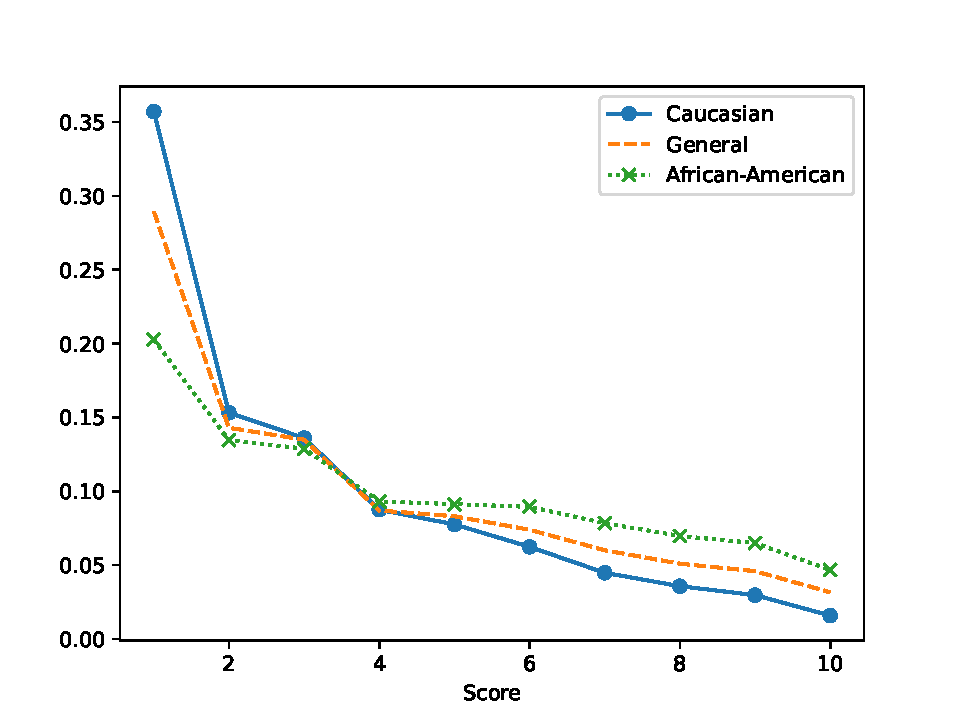
\includegraphics[width=\fwidth]{../figures/Scores-by-race}      
    \label{fig:risk-bias}
    \caption{Apparent bias in risk scores towards black versus white defendants.}
  \end{figure}
  \only<article>{ We can formalise the requirement for everybody to be
    equally, either with respect to the decisions, or with
    respect to the outcomes.  Decision parity is called \emph{equality
      of opportunity} and satisfies the following condition: }
  \begin{equation}
    \label{eq:equality-opportunity}
    \Pr_\param^\pol(a_t | z_t) =       \Pr_\param^\pol(a_t ).
  \end{equation}
  \only<article>{ Consequently, the action (risk score, in this case)
    is independent of the group.  In other words, the distribution of
    actions should be the same no matter what the group is. As we see
    in Figure~\ref{fig:risk-bias}, these distributions are quite
    different for the COMPAS example.  The curve for ``General'' corresponds to
    $\Pr_\param^\pol(a_t )$, while the other two curves correspond to
    $\Pr_\param^\pol(a_t | z_t)$ for $z_t$ being Caucasian and
    African-American respectively.
    
    \emph{Demographic parity} instead relates to outcomes. If this
    condition is satisfied, then the probability distribution of
    outcomes is independent of group membership:
    \begin{equation}
      \label{eq:eqality-outcomes}
      \Pr_\param^\pol(y_t | z_t) =       \Pr_\param^\pol(y_t ).
    \end{equation}
    As we can see in Table~\ref{tab:recidivism}, the recidivism rates are not the same across groups. Caucasian rates are nearly half those of African-Americans. While in this particular case, the judge's policy may not significantly affect the distribution, in other scenarios, such as loan decisions or university admissions they clearly do. 
    \begin{table}[h]
      \centering
      \begin{tabular}{r|r|r}
        African-American& General & Caucasian\\
        \hline
        10.8\% & 8.7\% & 6.5\% 
      \end{tabular}
      \label{tab:recidivism}
      \caption{Recidivism rates across ethnic groups.}
    \end{table}
    Given that Caucasians both have lower recidivism rates and lower scores than African-Americans, could this simply be because people with a higher chance of recidivism obtain higher scores? To explore this further, we need to look at some \emph{conditional} independence fairness notions. This measure how the actions and outcomes depend on each other when conditional on group membership.
  }
\end{frame}

\begin{frame}
  \frametitle{Calibration.}
  
  \only<article>{Let us first consider how well recidivism is
    predicted by the score across different groups. Perhaps partially
    explaining what we have seen before, the scores generated by the
    software seemed to be very predictive on whether or not defendants
    would re-offend, independently of their
    race. Figure~\ref{fig:imrs} shows that, if an individual obtains a
    high score then they are very likely to re-offend, and conversely,
    they are unlikely to re-offend when they have a low score. This
    dependence is similar for both groups.}
  \begin{figure}[H]
    \centering
    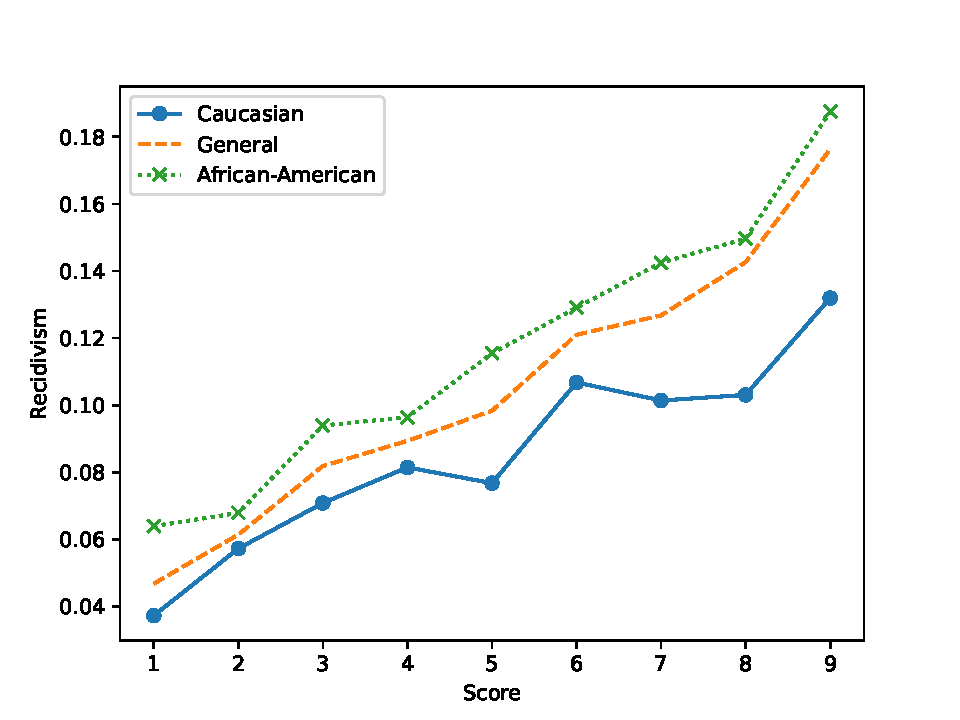
\includegraphics[width=\fwidth]{../figures/calibration-compas}
    \caption{Recidivism rates by risk score.}
    \label{fig:imrs}
  \end{figure}
  \only<article>{
    This concept can be quantified in terms of the conditional distribution of outcomes given the score:}
  \begin{equation}
    \Pr_\param^\pol(y_t | a_t, z_t) =       \Pr_\param^\pol(y_t | a_t).
    \label{eq:calibration}
  \end{equation}
  \only<article>{
    This means that $y_t$ is conditionally independent of $z_t$ given
    the score $a_t$. So, in some sense, the score is sufficient for us
    to predict the outcome, and knowing the race does not help us
    predict any better.
  }
\end{frame}

\begin{frame}
  \frametitle{Balance}
  \only<article>{While the system's predictions seem to be calibrated against the chance of recidivism, this does not mean that race plays no role. Figure~\ref{fig:imrs-risk} breaks down the population in people that re-offended and those that did. For each sub-population, we then plot the proportion of people receiving different scores by race. While people generally have a small probability of obtaining a high risk score, we see that Black defendants obtain much higher scores.}
  
  \begin{figure}[H]
    \centering
    \begin{subfigure}{0.45\textwidth}
      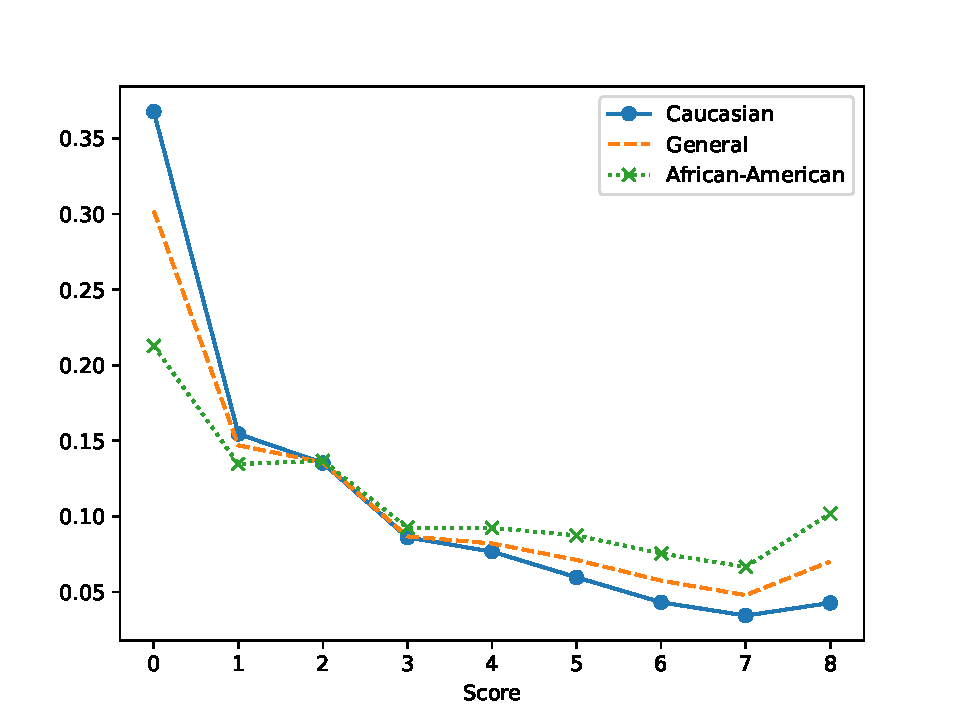
\includegraphics[width=0.95\textwidth]{../figures/balance-non-recidivism-compas}
      \caption{No recidivism}
    \end{subfigure}
    \begin{subfigure}{0.45\textwidth}
      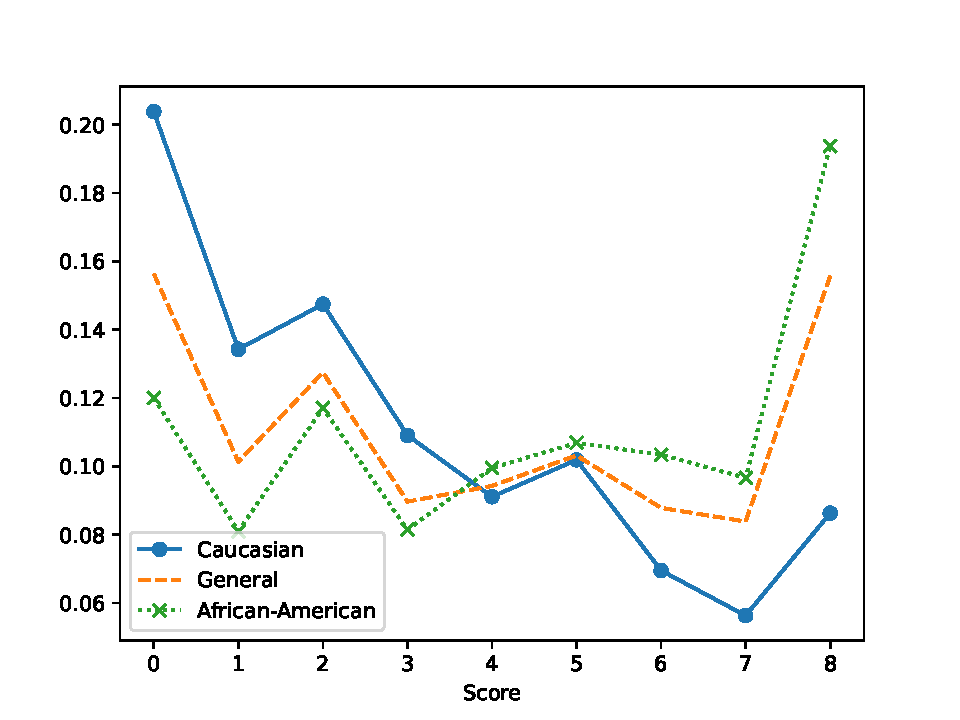
\includegraphics[width=0.95\textwidth]{../figures/balance-recidivism-compas}
      \caption{Recidivism}
    \end{subfigure}
    \caption{Score breakdown based on recidivism rates.}
    \label{fig:imrs-risk}
  \end{figure}
  \only<article>{
    Balance can also be interpreted as a probabilistic condition, of the following form:
  }
  \begin{equation}
    \Pr_\param^\pol(a_t | y_t, z_t) =       \Pr_\param^\pol(a_t | y_t).
    \label{eq:balance}
  \end{equation}
  \only<article>{
    Here we have that $a_t$ is conditionally independent of $z_t$
    given the outcome $y_t$. So, if we partition the population
    according to their outcome, we should find that given the outcome,
    the distribution of scores is the same no matter what their
    race. However, this is not what the example shows: there is a
    strong dependence on race.  }
  
\end{frame}


\begin{frame}

  \begin{example}[Classification]
    \only<presentation>{
      \begin{itemize}
      \item $y$: labels
      \item $a$: label prediction
      \item Here the outcome is independent of the action:
      \end{itemize}
    }
    \[
      \Pr_\param^\pol(y_t \mid a_t, x_t, z_t) =   \Pr_\param^\pol(y_t \mid x_t, z_t).
    \]

    Balance in classification:
    \begin{itemize}
    \item Equal false positive  rate:
      \[
        \Pr(a_t = 1 \mid y_t = 0, z_t = z) = r_{\textrm{FP}}, \qquad \forall z
      \]
    \item Equal false negative rate:
      \[
        \Pr(a_t = 0 \mid y_t = 1, z_t = z) = r_{\textrm{FN}}, \qquad \forall z
      \]
    \end{itemize}
  \end{example}
\end{frame}
\begin{frame}

  \begin{example}[Regression]
    \only<article>{
      We can also apply these ideas to regression problems. We are again
      asked to simply predict a latent variable $y$. For concreteness,
      assume $y \in \Reals$. Then, the decision space $\CA = \Reals$ as
      well. A standard utility function is the negative squared prediction
      error, so that $U(a, y) = - (a - y)^2$.
    }
    
    In this setting we can also relax our framework to work with
    expectations instead of probabilities. For example, calibration and balance can be written as the conditions:
    \[
      \E_\param^\pol(y_t | a_t, z_t) = \E_\param^\pol(y_t | a_t),
      \qquad
      \E_\param^\pol(a_t | y_t, z_t) = \E_\param^\pol(a_t | y_t),
    \]
    respectively.
    \only<article>{
      This is a useful definition in particular when our
      action is the assignment of a numerical score, as in the COMPAS
      recidivism example. However, this definition is weaker, as the
      expectations of two random variables can be equal when their
      distributions are different.
    }
  \end{example}
\end{frame}
\only<article>{
  \begin{theoryblock}{Conditional independence of $y, a$ given $z$.}
    There is another possibility, which we have not mentioned: What if $y, a$ are conditionally independent given $z$? Can we use that as a fairness criterion? If you spend a few minutes of thought, you will find that this condition should always when $y$ is not directly depend on $a$. In particular, consider the following graphical model where a person's features depend on their group membership. If there is no direct connection between $y, a$, then they are already conditionally independent given the group.
    \begin{tikzpicture}
      \node[RV] at (0,0) (z) {$z$};
      \node[RV] at (1,0) (x) {$x$};
      \node[RV] at (2,-1) (a) {$a$};
      \node[RV] at (2,1) (y) {$y$};
      \draw[->] (z) to (x);
      \draw[->] (x) to (a);
      \draw[->] (x) to (y);
    \end{tikzpicture}
  \end{theoryblock}
}

\section{Individual fairness}
\only<presentation>{
  \begin{frame}
    \centering
    {\Huge Individual fairness}
  \end{frame}
}
\only<article>{ An altogether different type of fairness concept is
  individual fairness. This is linked to the notion of meritocracy, i.e.
  that ``better'' people should have ``better'' outcomes. But what do
  we mean by better? This depends strongly on the context: people that
  are better than others in one respect might be worse in another,
  i.e. student A might be better in Math than student B, but worse in
  History, and student A might prefer the Math department to the
  History department and vice-versa.  In addition, what is better for
  a person is a direct result of that person's preference.  An
  alternative concept for individual fairness is treating similar
  people similarly. Then the question is, what do we mean by similar?
  Again, in some contexts different features of individuals might be
  more important as a way to measure similarity: when considering
  university applicants, their grades are probably more important to
  determine which student should be accepted to a degree program,
  rather than their eye colour.

  A lot of the variables we might be interested in are not
  observed. For example, we might want to know the true potential and
  skill of a student in Math. However, the only thing we have is their
  exam or high-school grades, which are mere proxys for their true
  skills. While one of the easiest ways to deal with meritocracy is to
  define worth precisely respect to those observed variables, it is a
  good idea to use inferred measures of worth if possible. However,
  this requires building some type of model.

  Finally, even though we are making decisions about individuals,
  frequently these are made about multiple individuals at once. This
  is is the case in university placements, for example, where
  thousands of students submit their preferences for different
  university programmes, and then they are placed depending on their
  own preferences, as well as their grades. Thus, the problem faced by
  the decision maker is not a simple classification, but rather a
  matching problem.
}

\begin{frame}
  \begin{block}{Main variables for individual fairness.}
    \only<article>{To define fairness with respect to a decision maker, we need to specify what is observed by the decision maker, and what the decision maker performs.}
    \begin{itemize}
    \item $x_i \in \Reals^d$: Individual features. \only<article>{That's what we observe about the $i$-th individual. In the university setting this would correspond to their grades and other personal information.}
    \item $w_i \in \Reals$: Individual worth. \only<article>{This can be taken to mean how well the individual is expected to perform in university, e.g. their expected grade. However, this quantity is not directly observed.}
    \item $u_i : \CA \to \Reals$: Individual utility. \only<article>{This is how much the individual gains by the decision. For simplicity, we can imagine that $i$ is only impacted by the decision regarding them, rather than anybody else, so we can just define a function $u_i(a_i)$ instead.}
    \item $a \in \CA$: Action taken by the decision maker. \only<article>{For
        example, $a$ could specify which applicants are admitted to
        university, with $a_i$ specifying the university to which 
        applicant $i$ is admitted.}
    \item $\pol$: The decision maker's policy for making decisions.
      \only<article>{This is defined as $\pol(a | x)$, the probability of a decision given the features of the population. In some settings, the policy makes decisions for each individual separately. Then we can define their policy $\pol(a_i | x_i)$ in terms of individual decisions $a_i$ and observations $x_i$. This also means that the decision about any one individual does not depend on either the features of or the decisions for other individuals:
        \[
          \pol(a | x) = \prod_i \pol(a_i | x_i). 
        \]
        However, in many cases, such as in university admissions, we make our decisions about everybody at the same time. Then the above independence condition does not hold, and the decision maker's choice depends on everybody's observations.}
    \end{itemize}
  \end{block}
\end{frame}

\subsection{Meritocracy.}

\only<article>{Let us first discuss the concept of meritocracy as it
  relates to an individual's inherent worth. The assumption here is
  that individuals can be ranked in terms of their worth, so that
  individuals with more worth are deserving of higher rewards. Of
  course, this idea is only easy to work with when we know the worth
  of each individual, as well as how much each one values possible
  rewards.

  In addition, we have to have a notion of the worth of rewards. The
  simplest assumption is that for any pair of possible rewards
  (e.g. university placements), everybody prefers one of them to the
  other. However, we do not expect everybody to have the same
  preferences. Indeed, in university placements, each student
  typically submits and ordered list of preferences and they are
  matched to programs according to their preferences and their
  grades.

  In the definition below, we assume that every individual has a
  specific, invariant, inereht worth. They also have a clear
  preference over the decision maker's actions.
}


\begin{frame}
  \frametitle{Meritocracy for given utilities and worths.}
  \only<article>{ The following definitions are applicable for any
    type of decision making over individuals. An important point is
    that there is a distinction between decisions being fair and
    policies being fair. Requiring that individual decisions satisfy a
    fairness constraint is much stricter than a similar requirement
    for policis. }
  \begin{definition}
    A \textbf{decision} $a$ is \textbf{fair} if, for all $i,j$, we have $w_i > w_j \Rightarrow u_i(a) \geq u_j(a)$.
  \end{definition}
  \only<article>{In the above definition, a person with a higher worth than another is guaranteed to obtain at least as good an outcome as another person of lower worth. If we think about a single decision affecting multiple individuals, then such a fairness property is hard to satisfy: in some cases there may not exist any such fair decision, as shown in the example below.}
  \begin{example}
    \begin{tabular}{c||c|c|c}
      $w$ &  &  $a = 0 $ & $a = 1$\\
      \hline
      1  & $u_1$ & 0 & 1\\
      0  & $u_2$ & 1 & 0
    \end{tabular}
  \end{example}
\end{frame}
\begin{frame}
  \begin{definition}
    A \textbf{policy} $\pol$ is \textbf{fair} if, for all $i,j$ it holds that: $\E_\pol [u_i | w] > \E[u_j | w] \Rightarrow w_i > w_j$.
  \end{definition}
  
  \only<article>{ Let us consider problems where the decision maker
    has a binary choice, e.g. to accept or reject a loan
    application. In particular, the decision rule may be restricted so
    that the decision has to depend only on a \emph{score}, e.g. the
    credit score. Let $w_i$ be the score of the $i$-th
    individual. Typically, the decision $a_i$ about an individual $i$
    does not depend on the decision about any other individual. Hence,
    the decision rule can be factorised as
    $\pol(a | w) = \prod_i \pol(a_i | w_i)$. This is typically the
    case when individuals appear sequentially, and we must make a
    decision for each one of them in turn, as long as the decision
    rule $\pol$ remains fixed.
    
    However, in some cases $\pol$ itself depends on a population of individuals. This is the case in cohort selection, when we need to select some individuals from a set.
  }


  \begin{example}[Ranking and top-$k$ cohort selection.]
    \only<article>{
      In this setting, we assume we have a set of $n$
      individuals, with the $i$-th individual receiving an evaluation
      $w_i$. We need to choose individuals from the set so that
      $a_i = 1$ if we select an individual, and $0$ otherwise. We can
      assume that all individuals prefer being selected.  The
      selection algorithm $\pol$ creates an allocation
      $a=(a_1, \ldots, a_n)$. A simple way to perform the allocation
      to first rank the individuals so that $w_{i} > w_{i+1}$. We then
      can assign $a_i=1$ for all $i \leq k$.
    }
    \only<presentation>{
      \begin{itemize}
      \item $n$ individuals
      \item $i$-th individual receiving an evaluation
        $w_i$.
      \item $a_i = 1$ if we select an individual, and $0$ otherwise.
      \item Ranked selection algorithm $\pol$: first rank the individuals so that $w_{i} > w_{i+1}$. We then     can assign $a_i=1$ for all $i \leq k$.
      \end{itemize}
    }
  \end{example}
\end{frame}
\only<article>{
  This, however, creates a problem. What if the $k$-th individual has value $w_k$, but there exist more individuals of equal value, so that e.g. $w_{k+1} = w$? Due to our constraint on only selecting $k$ individuals from the set, we now have a problem: if we select $k$ and not $k+1$, we are treating the individuals differently, even though their characteristics are exactly the same. The simplest way to fix that is to choose between $k$ or $k+1$ with probability $1/2$ each. The same problem occurs when we want to match multiple individuals to one of many possible allocations, as is done in university entrance. The obvious solution there is also randomisation. Even though some people find randomisation fundamentally unfair, it is the only method offering equitable treatment (though not equitable outcomes) for indistinguishable individuals.
}



\end{document}

%%% Local Variables:
%%% mode: latex
%%% TeX-engine: xetex
%%% TeX-master: t
%%% End:
